\section{Programmable Storage}
\label{sec:progly}

Common workarounds when application requirements are not met
by an underlying storage system roughly fall into three categories:

{\bf ``Bolt-on services''} improve performance
or enable new features, but come at the expense of additional hardware, software
sub-systems, and dependencies that must be managed, as well as trusted.
For instance, such classes of limitations inspired many extensions to Hadoop
~\cite{bu:vldb2010-haloop, ekanayake:hpdc2010-twister,
ekanayake:escience2008-eglmapreduce, mihailescu:hotstorage2012-mixapart}.

{\bf Application changes} introduce data management intelligence or integrate
domain-specific middleware into an application.  When application changes
depend on non-standard storage semantics (e.g. relaxed POSIX file I/O or
MPI-IO hints) the resulting coupling can be fragile.  For example, both
SciHadoop~\cite{buck:hpc2011-scihadoop} and
Rhea~\cite{gkantsidis:nsdi2013-rhea} do an excellent job of partitioning data
in Hadoop applications, but may not withstand the test of time for future
workloads, since the partitioning is specific to the use case. Approaches to
I/O optimization in middleware (e.g.  MPI-IO) take advantage of an
application's structured and partitioned data model, but face portability
challenges when mapping parallel I/O onto a bytestream. The challenge is, in
part, due to the wide range of optimization strategies that are dependent on
low-level storage system \emph{magic numbers} for optimal data partitioning,
distribution, and alignment. The PLFS file system takes an approach of
virtualizing the POSIX byte stream over a set of logs to address this
issue~\cite{plfs}.

{\bf Storage system modifications} are often a last resort because such
heavyweight solutions range from merely changing the underlying system to
designing entirely new systems. This approach requires at a minimum, a certain level of
access to modify the system, significant cost, domain knowledge, and extreme care when building or
modifying critical software that can take years of code-hardening to trust.
For example, HDFS fails to meet many needs of metadata-intensive
workloads~\cite{shvachko:login2012-hdfs-scalability}.  This has lead to
modifications to its architecture and API~\cite{balmin:sigmod2012-clydesdale}
to improve performance.

Rather than relying on storage systems or applications to change, Malacology
exposes data management services already present in the underlying system,
which can be re-used to avoid code duplication and reliance on external
services.

\subsection{The Malacology Approach}
\label{mala}

Malacology is a prototype programmable storage system based on Ceph that
improves the development experience of co-designing applications and storage
systems by exposing common internal storage services for
re-use~\cite{sevilla:eurosys17}. Figure~\ref{fig:malacology} shows the
architecture of Malacology, along with the set of services that are exposed,
such as domain-specific object interfaces, cluster-level metadata management,
and load-balancing. While Ceph natively exposes file, block, and object
abstractions, Malacology demonstrates the construction of two real-world
services using only the composition of existing interfaces present in Ceph.

\begin{figure}[t]
\centering
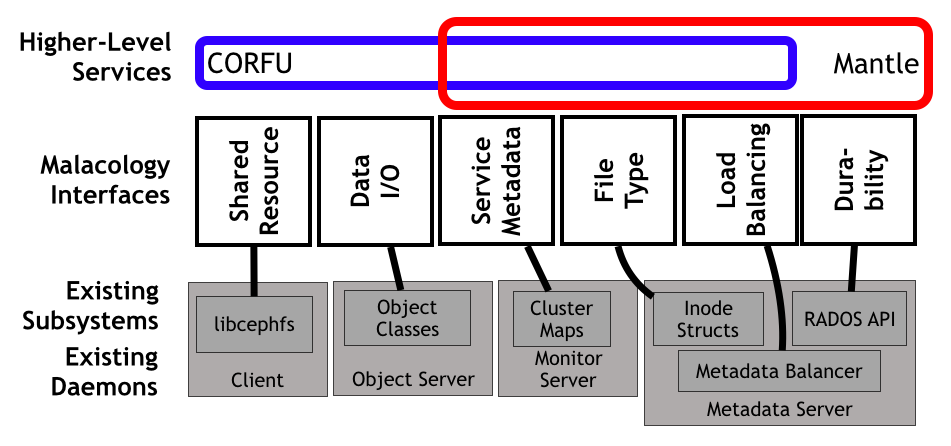
\includegraphics[width=1.0\linewidth]{implementation-overview.png}
\caption{Malacology implementation in Ceph. Existing sub-systems are composed
    to form new services and application-specific optimizations.}
\label{fig:malacology}
\end{figure}

One of these synthesized interfaces is a high-performance distributed
shared-log
based on the CORFU protocol~\cite{balakrishnan:nsdi12}.  While CORFU can
be a stand-alone system, Malacology is capable of instantiating the same storage
abstraction and approximating the same optimizations. High-performance in CORFU
is achieved in part through the use of a soft-state network-attached counter.
Malacology approximates this optimization using the capability-based caching
mechanisms in the Ceph distributed file system, modeling the counter as a
shared resource (i.e. file metadata). Additionally, the co-designed device
interfaces used in CORFU are critical to the safety of the protocol, and are
replicated in Ceph using custom software-based interfaces to storage objects.

While powerful, storage interface construction in Malacology (Data I/O interface in
Figure~\ref{fig:malacology}) is a double-edged
sword. The narrowly-defined interfaces dominating systems today have been a
boon to developers by limiting the size of the design space where applications
couple with storage, allowing systems to evolve independently. Programmable
storage lifts the veil on the system and, with it, forces developers of
higher-level services to confront a large and expanding set of possible
designs.
